\section{Parameter Estimation}\label{sec:analysis}

A number of parameters can be tweaked to change the patch matching and storage, and different choices may be appropriate for different applications and performance requirements (both quantitative and qualitative). These parameters include the size of the input images, the size of the patches extracted, the sampling strategy used to seed the dictionary, the distance metric and thresholds used to compare patches, as well as the parameters required for indexing and retrieving patch matches (approximate nearest neighbors). Here we discuss some of the parameter choices made and the experiments that lead up to these choices. Other possible choices are discussed in Sec.\ref{sec:futureext}.

Our quantitative performance metrics involve examining how the patch dictionary size grows with the addition of new images to the database (the growth function and rate) and the compression ratio per image (viewed as a distribution over compression ratios and summarized as the average compression ratio). Qualitative evaluations involve determining whether a human can spot compression artifacts and how salient they are in the images. The authors of this paper manually examined images reconstructed from the dictionary patches. A crowdsourced evaluation strategy involving Amazon's Mechanical Turk may be appropriate for larger-scale studies, but was beyond the scope of this paper.

There will always be a trade-off between compression benefits (storage: patch dictionary size and speed: image reconstruction time) and reconstruction quality. For many computer vision tasks including scene recognition (and thus retrieval), imperfect reconstructions with artifacts may not be a problem as long as the overall scene structure does not change. For instance, \cite{tiny_images} has shown that with images of pixel dimension 32x32, humans are already able to achieve over $80\%$ scene and object recognition rate. See fig.\ref{fig:badrecon} for a demonstration of an image that has serious reconstruction artifacts, but when down sampled (to a thumbnail), they become insignificant, and thus do not necessarily impair visual recognition.

 \begin{figure}
%\hspace{-25mm}
\centering
(a) 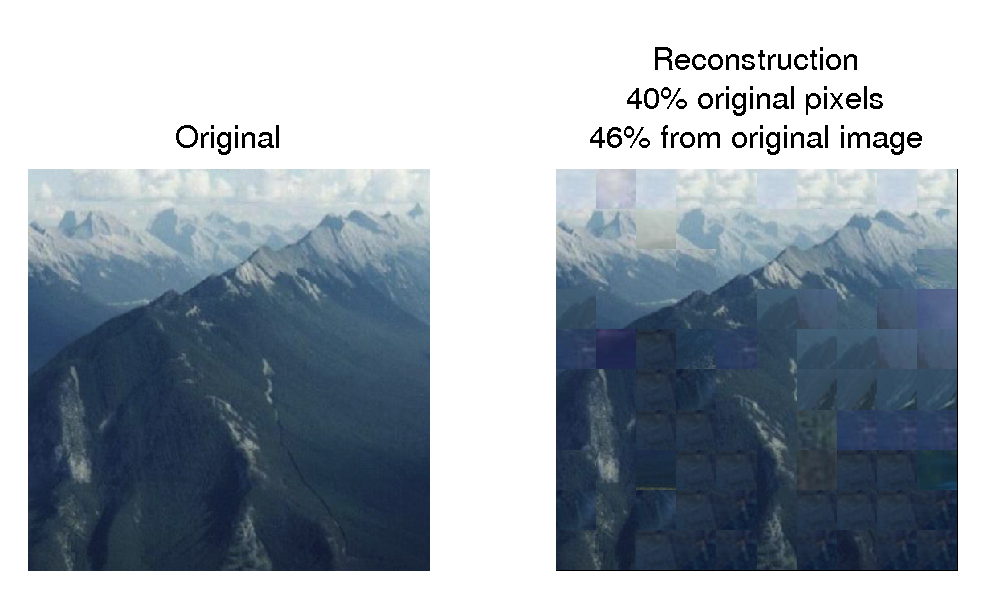
\includegraphics[width=0.9\linewidth]{Figures/184.png}
(b) 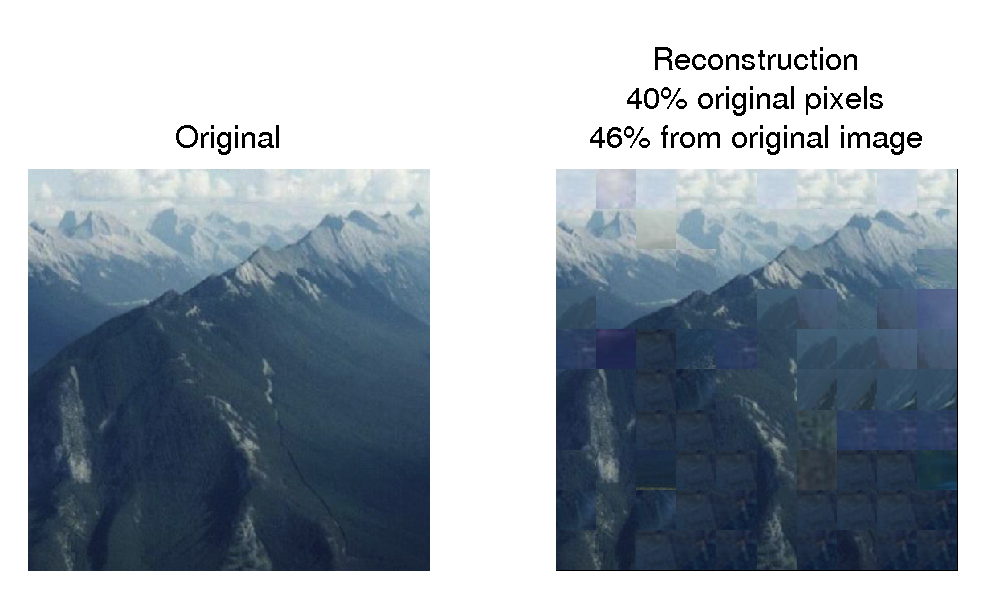
\includegraphics[width=0.4\linewidth]{Figures/184.png}
\caption{For demonstration purposes only, we choose a large patch size and low distance threshold. (a) Under these parameters, the original image is reconstructed to take up only $40\%$ of its original size (in pixels). The $60\%$ of the patches that have been replaced come either from the same image ($46\%$ of them), or from other images (the remaining $64\%$). (b) Notice that when the size of the image and its reconstruction are halved, the artifacts already become visually insignificant, and would not impair a scene recognition or search task. }
\label{fig:badrecon}
\end{figure}

 \begin{figure}
%\hspace{-25mm}
\centering
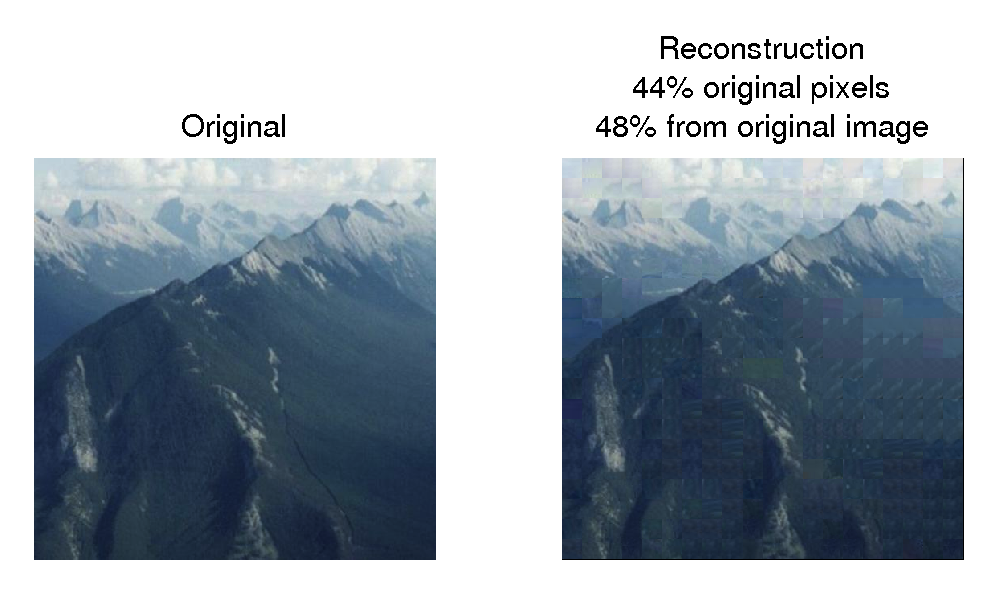
\includegraphics[width=0.9\linewidth]{Figures/184_25.png}
\caption{Compare this image reconstruction, computed with a dictionary of $25\times 25$ pixel patches with the reconstruction in fig.\ref{fig:badrecon}, computed with $50\times 50$ patches. In both cases, a similar threshold is used (scaled to the patch size, as discussed in sec. \ref{sec:simthresh}) but the visual artifacts are less noticeable because smaller patches have less contained structure, and are more likely to be homogenous in appearance.}
\label{fig:patchsize}
\end{figure}


%\subsection{Quality Metrics}\label{ssec:qual-met}
%There are many possible formulations of these quality constraints; we detail those that we considered for this paper in section TODO.  Beyond mathematical metrics, subjective methods are also interesting to consider for formulating the quality constraints; one could imagine a scenario in which image quality is assessed by humans through a crowdsourced system, perhaps using an engine such as Amazon's Mechanical Turk TODO: cite.  We consider such subjective similarity metrics outside the scope of this paper and focus on the mathematical metrics for now.

%We wish to construct a database that trades off minimizing the amount of required space with maximizing read and write speeds of the data.

\subsection{Patch Size}
\label{sec:patchsize}

%TODO(Zoya,Andrew): tradeoffs for patch size

%\begin{edit}
%(written by Andy): I think this should be moved earlier, after which the analysis is added.  Maybe we should add some stuff on the "quality gains" and add a plot for that, but there's not much we can probably do until later.
%\end{edit}

At larger patch granularities, each patch contains more image structure, and thus the probability that another patch contains the same or similar image content decreases with the number of pixels in a patch. At larger granularities it becomes increasingly harder to find matching patches in the patch dictionary, and the closest matching patches for textured regions might introduce artifacts (see fig.\ref{fig:patchsize}). At the same time, patches that are too small do not offer as efficient a compression strategy. We must balance the costs of storing pointers to patches for each image in our database, as well as all the patches themselves, against the costs of storing the images in their original form. This calculation is investigated further below. 

%In the extreme case, a patch is equal to one pixel, so the probability of an identical color patch is $\frac{1}{255^3}$, assuming 3 color channels. This value is multiplied by itself as many times as there are pixels in a patch to find an identical patch. For our application, we are interested in similar patches, rather than identical ones (see sec.\ref{sec:simthresh}), and so this probability is higher but bounded by this value, and similarly scales with patch size. 

\subsubsection{Cost Evaluation}
\label{sec:costeval}

Assume, as before, that $d$ is the number of patches in \texttt{patch\_dict}.  In practice, $d$ is a function of the number of images added to the database as well as the distance function $S$ and threshold $T$.  We further assume that each pixel requires 3 bytes to store and that each pointer is 8 bytes (a standard integer for a 64-bit system).  Then, with $k$ images in the database, the full cost to store all the original images (no patch-based compression scheme) in our database is:

\begin{equation}
	 c'(k, m) = 3  k  m^2
\end{equation}

\noindent In the case where we store pointers to patches, we have two tables: one table to store pointers to dictionary patches, and a second table to store the dictionary patches themselves.  Under this ``patch pointer" scheme, with $k$ images and $d$ patches, the cost $c$ to store all the images in our database is:

\begin{equation}
	c(k, d, m, n) = 8 k \left(\frac{m}{n}\right)^2 + 3  d  n^2
\end{equation}.

The first term is the cost of storing the pointer data, while the second term is the cost of storing the patches themselves.  The $8$ constant comes from the fact that we are dealing with very large image and patch tables ($ > 2 \times 10^9$ patches), and thus a \texttt{bigint} type is required to store the patch references.

Given these two equations, for a fixed $m$ and $n$, we can easily see that our compressive scheme becomes more space-efficient that storing the original images when:

\begin{equation}
	d < \frac{m^2 (3n^2 - 8) k}{3n^4}
\end{equation}

As long as we choose a distance threshold such that new image patches get added at a rate that guarantees this inequality is satisfied, our compressive method of image storage will save space.  Figure \ref{fig:optcost} shows an example of how the optimal storage cost changes with different patch and image counts, where the optimal cost is defined as $c_{opt} = \min{(c, c')}$; in other words, storing the images using the less expensive method. See fig. \ref{fig:optcost}.

 \begin{figure}
%\hspace{-25mm}
%\centering
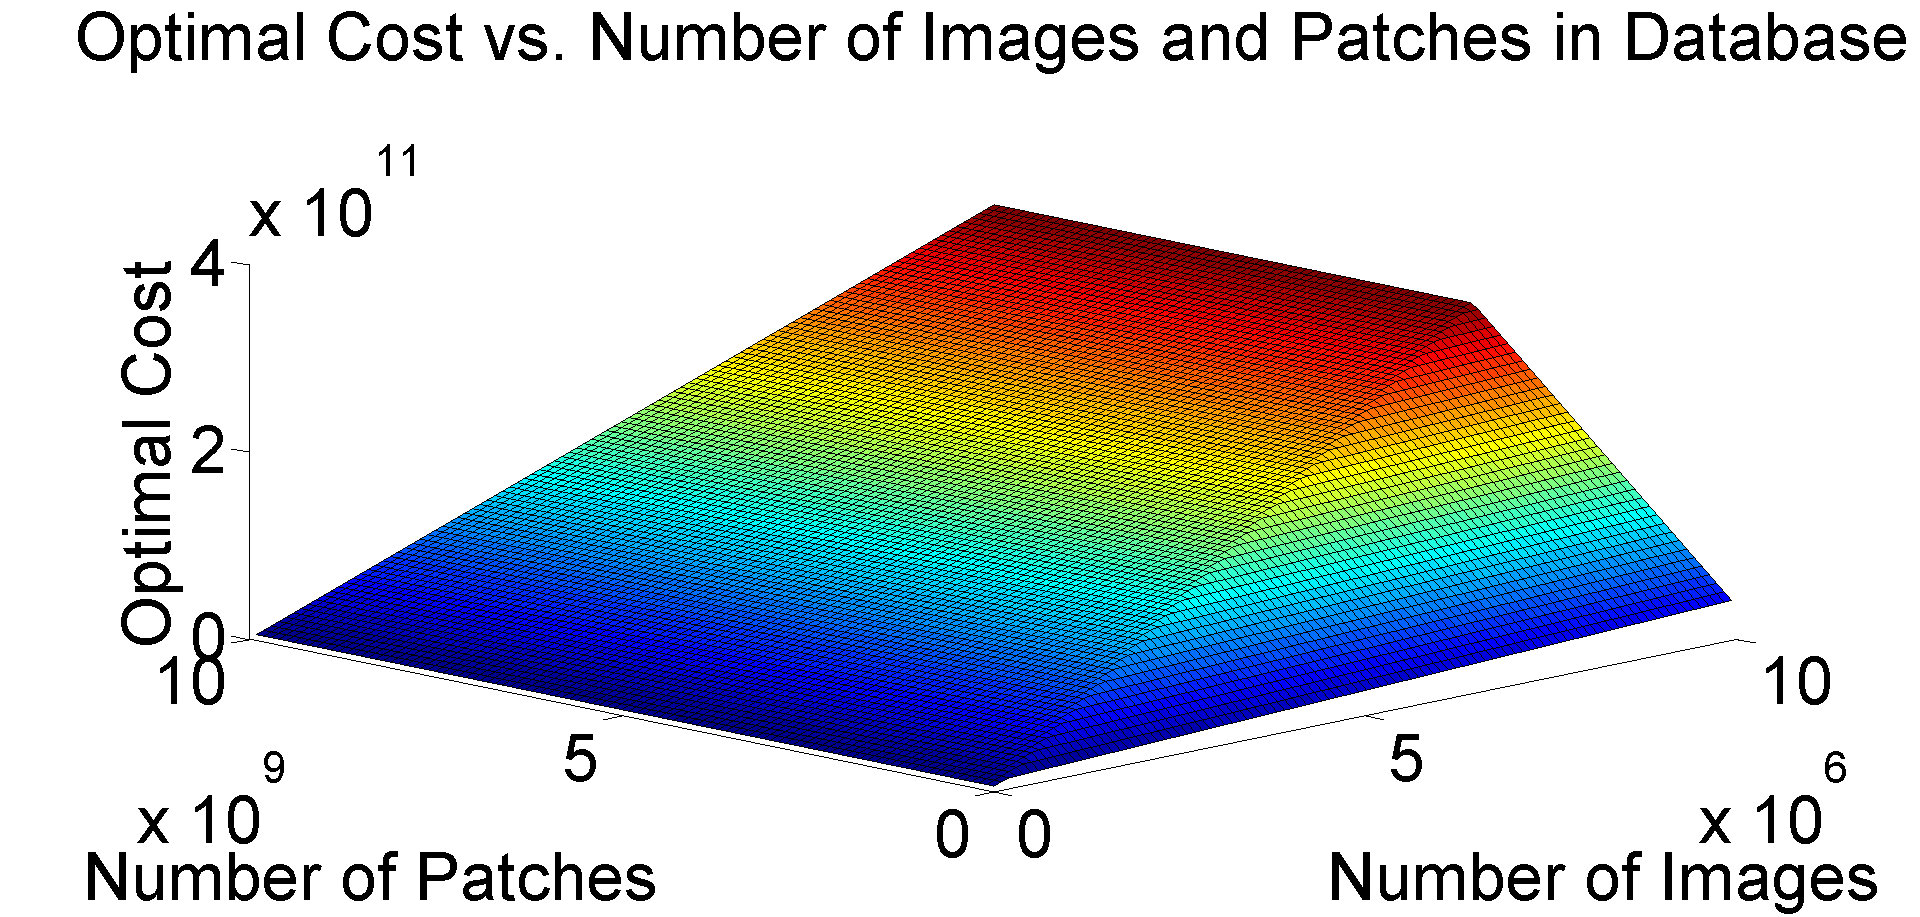
\includegraphics[width=1\linewidth]{Figures/PatchCosts.png}
\caption{A graph demonstrating how $c_{opt}$ changes with $k$ and $d$ for $m=100$ and $n=10$.  Note the line of discontinuity where $d = 357.3 k$ - this is the line where the costs of $c$ and $c'$ intersect.}
\label{fig:optcost}
\end{figure}


\subsection{Sampling strategies}
\label{sec:sample}

A patch dictionary can be built up incrementally, adding new patches as new images are added to the database. A potential problem with this approach is that image reconstruction quality will tend to decrease with the order in which images are added, such that images added to the database earlier will tend to have more patches that correspond to them (see Fig.\ref{fig:sampStrategy} for an example). A strategy with a more even distribution of reconstruction quality over images involves starting with a batch of images, and seeding the dictionary by randomly sampling patches from a set of images from the batch. This is the strategy we employ. 

 \begin{figure}
%\hspace{-25mm}
%\centering
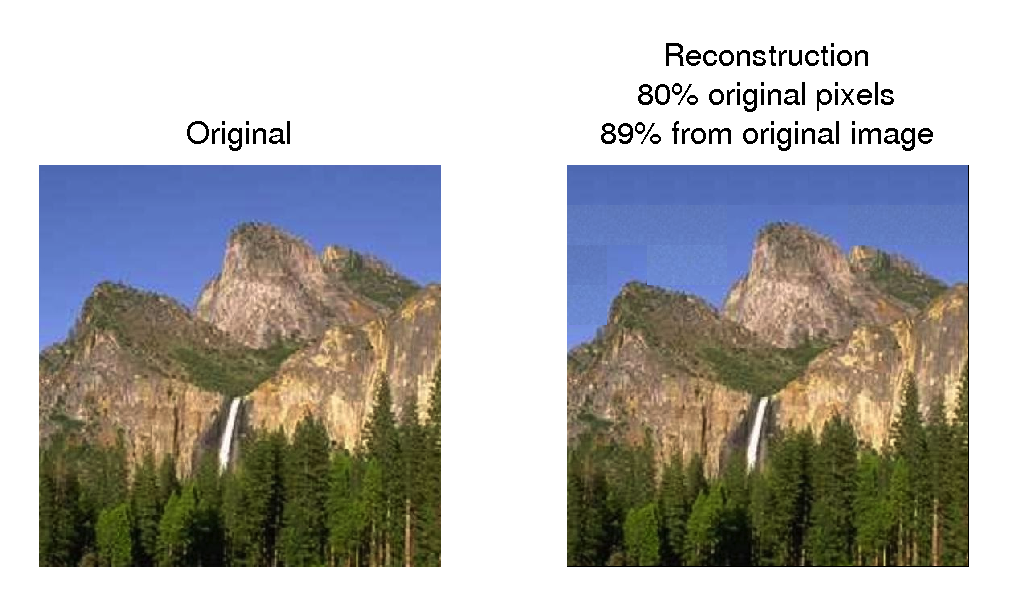
\includegraphics[width=0.9\linewidth]{Figures/009.png}
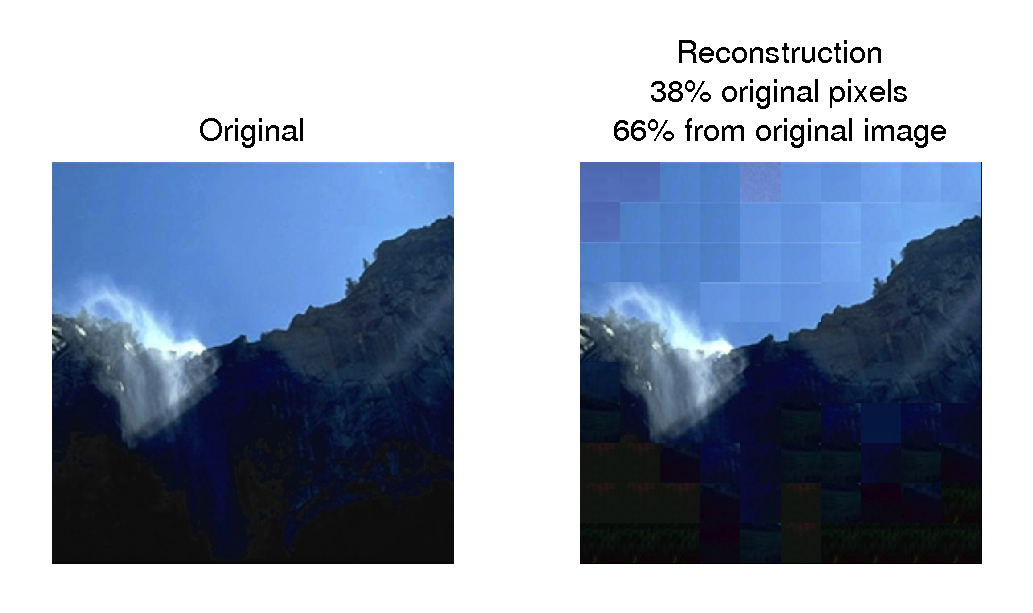
\includegraphics[width=0.9\linewidth]{Figures/014.png}
\caption{Example of a biased patch dictionary construction strategy, leading to non-uniformity in image reconstruction quality. Images added to the database earlier (top row) are better reconstructed (due to more patch samples in the database) than images added later (bottom row), constrained to be constructed out of patches added initially. The sky pixels in the image added later are borrowed from sky pixels of other images ($44\%$ of the pixels in this image come from other images, compared to only $11\%$ in the image on the first row). Note: here we use a very high patch distance threshold and large patch size for demonstration purposes only, to emphasize the artifacts created.}
\label{fig:sampStrategy}
\end{figure}


\subsection{Distance Function}
\label{sec:simthresh}

Many image (more specifically, patch) distance functions are possible, each with its own distinct set of parameters that can be tweaked for the required application. Because we are dealing with patches of a size specifically chosen to increase within-patch homogeneity, we do not consider cases of patches containing objects (the most we expect is an object boundary or simple texture), and thus do not need to consider complex image similarity/distance functions (involving SIFT, GIST, and other computer vision features). We can constrain ourselves to color distance, and split a patch $P_i$ into 3 LUV color channels: $P_i(L), P_i(U), P_i(V)$. 

Then we consider two patches $P_i$ and $P_j$ similar when, given $n\times n$ patches, all of the following are true:
\begin{align*}
\frac{1}{n^2}||P_i(L) - P_j(L)||^2 < T_1 \\
\frac{1}{n^2}||P_i(U) - P_j(U)||^2 < T_2 \\
\frac{1}{n^2}||P_i(V) - P_j(V)||^2 < T_3
\end{align*}

The $\frac{1}{n^2}$ term allows us to normalize for patch size, so that the threshold values chosen becomes independent of patch size. Here we constrain the average distance value of all the pixels in a patch to fit a threshold, whereas it is possible to have alternative constraints (where instead of the average, the maximal pixel difference or the variance of the pixel differences or some other measure over pixels in a patch, is compared to a threshold).

Note additionally that if instead we fix a single threshold for the sum of the Euclidean differences in the 3 color channels as in: 
\begin{displaymath}
\frac{1}{n^2}[||P_i(L) - P_j(L)||^2 + ||P_i(U) - P_j(U)||^2 + ||P_i(V) - P_j(V)||^2] < T
\end{displaymath}
then the similarity in one color channel may compensate for the difference in another, producing skewed results (see fig.\ref{fig:colProblem}).

Multiple color channels are possible, but we choose to work in the (CIE)LUV color space, which is known to be more perceptually uniform than the standard RGB color space~\cite{kekre2012performance}. Additionally, our formulation makes it possible to impose separate distance thresholds on each of the color channels ($T_1,T_2,T_3$). However, for simplicity, we set $T_1=T_2=T_3=T$, where the choice for the value of $T$ is described next.

\subsection{Distance Threshold}

Choosing a threshold $T$ requires weighing the quantitative benefits of compression with the qualitatively poorer image reconstructions. We ran a number of experiments, varying the threshold, and quantitatively and qualitatively examining the results. We rescale each color channel to be between 0 and 1, in order to choose a threshold $T$ that is bounded by these values (and is independent of color representation). In fig. \ref{fig:perfGraphs} we plot a few small experiments (with 200 images) for demonstrative purposes. The images were $500\times 500$ pixels, and the patch size was $25\times 25$. We chose this patch size due to the discussion in \ref{sec:patchsize}. Below we consider a number of quantitative indicators for patch compression. 

In the set of graphs in the first column of fig. \ref{fig:perfGraphs}, we plot in blue the dictionary size against the number of images added to the database. We compare this to the total number of patches that would have been stored if no compression scheme was utilized (red dotted line). We can see that for all choices of threshold, the size of the patch dictionary grows slower than the total number of patches that would need to be added if all images were stored along with their original patches. The gap between the blue and red dotted lines is a measure of the storage savings. As the threshold becomes more stringent, the blue line approaches the red dotted line. Note additionally that as the threshold becomes smaller, patches are more likely to be reused from the same image than from other images when compressing an image, because only patches from the same image will be similar enough to other patches from this image.

The second column of fig. \ref{fig:perfGraphs} contains histograms indicating how many images contributed different amounts of new patches to the patch dictionary. When the threshold is very small (as in the histogram in the last row) more of the images contribute most of their patches (380-400 new patches added to the patch dictionary per image). Note additionally that the small number of images that are contributing 0 new patches to the dictionary account for the $10\%$ duplicates that are present in the SUN database (more about this in sec. \ref{sec:apps}).

The third column of fig. \ref{fig:perfGraphs} contains an insertion history: for each image inserted into the database, we track how many of its patches were added to the patch dictionary. We can see that as the patch distance threshold decreases, most images contribute most of their patches. This provides similar information as the histogram (which is merely the cumulative), but allows us to monitor any temporal changes. The spikes to 0 in this graph are indicative of duplicate images, and are discussed further in sec. \ref{sec:apps}.

In the final column of fig. \ref{fig:perfGraphs}, we see a sample image reconstruction. We can see that the reconstruction quality increases, and visual artifacts decrease, as the distance threshold decreases (becomes more stringent). At some point in the middle, the reconstruction is already indistinguishable from the original, but with significant database compression benefits. Thus, for further analysis we consider the threshold $T=8$ (recall that this is per color channel, and is independent of patch size).
%Thus, given two patches $P_i$ and $P_j$, we can measure their similarity in a given color channel by taking the Euclidean distance of the color values across all the pixels. 

%where a patch is a collection of pixels, each of which is defined to be a triplet of integer values, assuming a 3-D color space. For a patch $P_i$, let us define its 3 color channels to be: $P_i(1), P_i(2), P_i(3)$.

 \begin{figure}
%\hspace{-25mm}
%\centering
(a)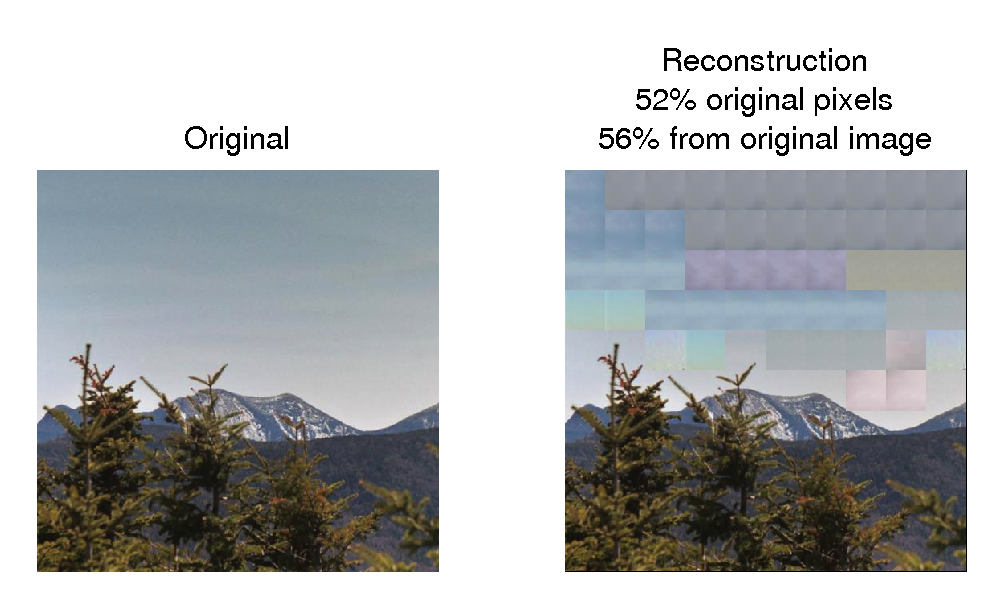
\includegraphics[width=0.9\linewidth]{Figures/197.png}
(b)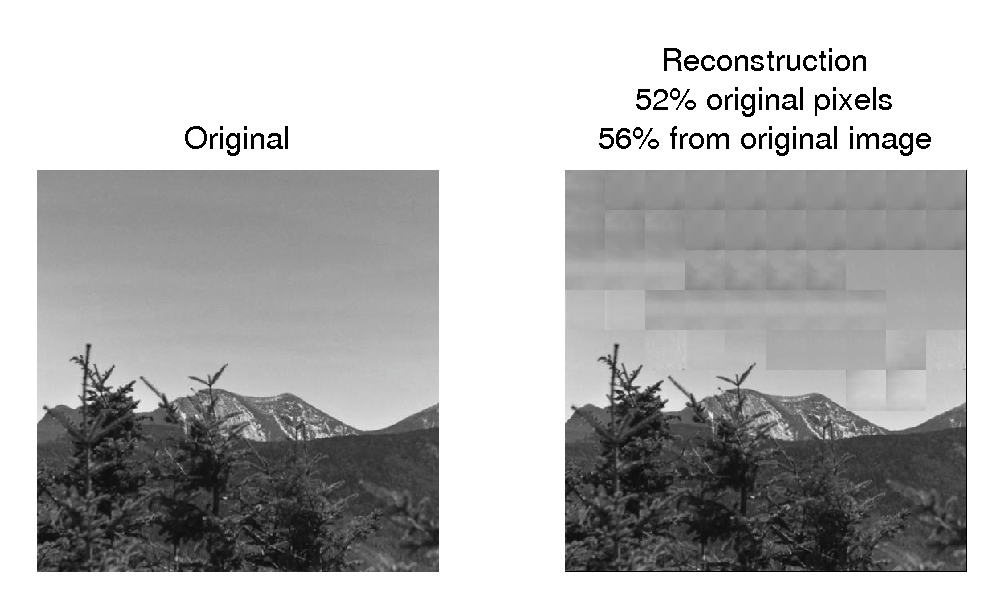
\includegraphics[width=0.9\linewidth]{Figures/197_bw.png}
\caption{This is what happens when we do not separately constrain each of the color channels to match. We have patches that are (a) the wrong color and produce visible visual artifacts, while (b) matching in terms of general hue (average of the color channels). Again, the patch size and distance threshold were chosen to emphasize the artifacts.}
\label{fig:colProblem}
\end{figure}

 \begin{figure*}
%\hspace{-25mm}
%\centering
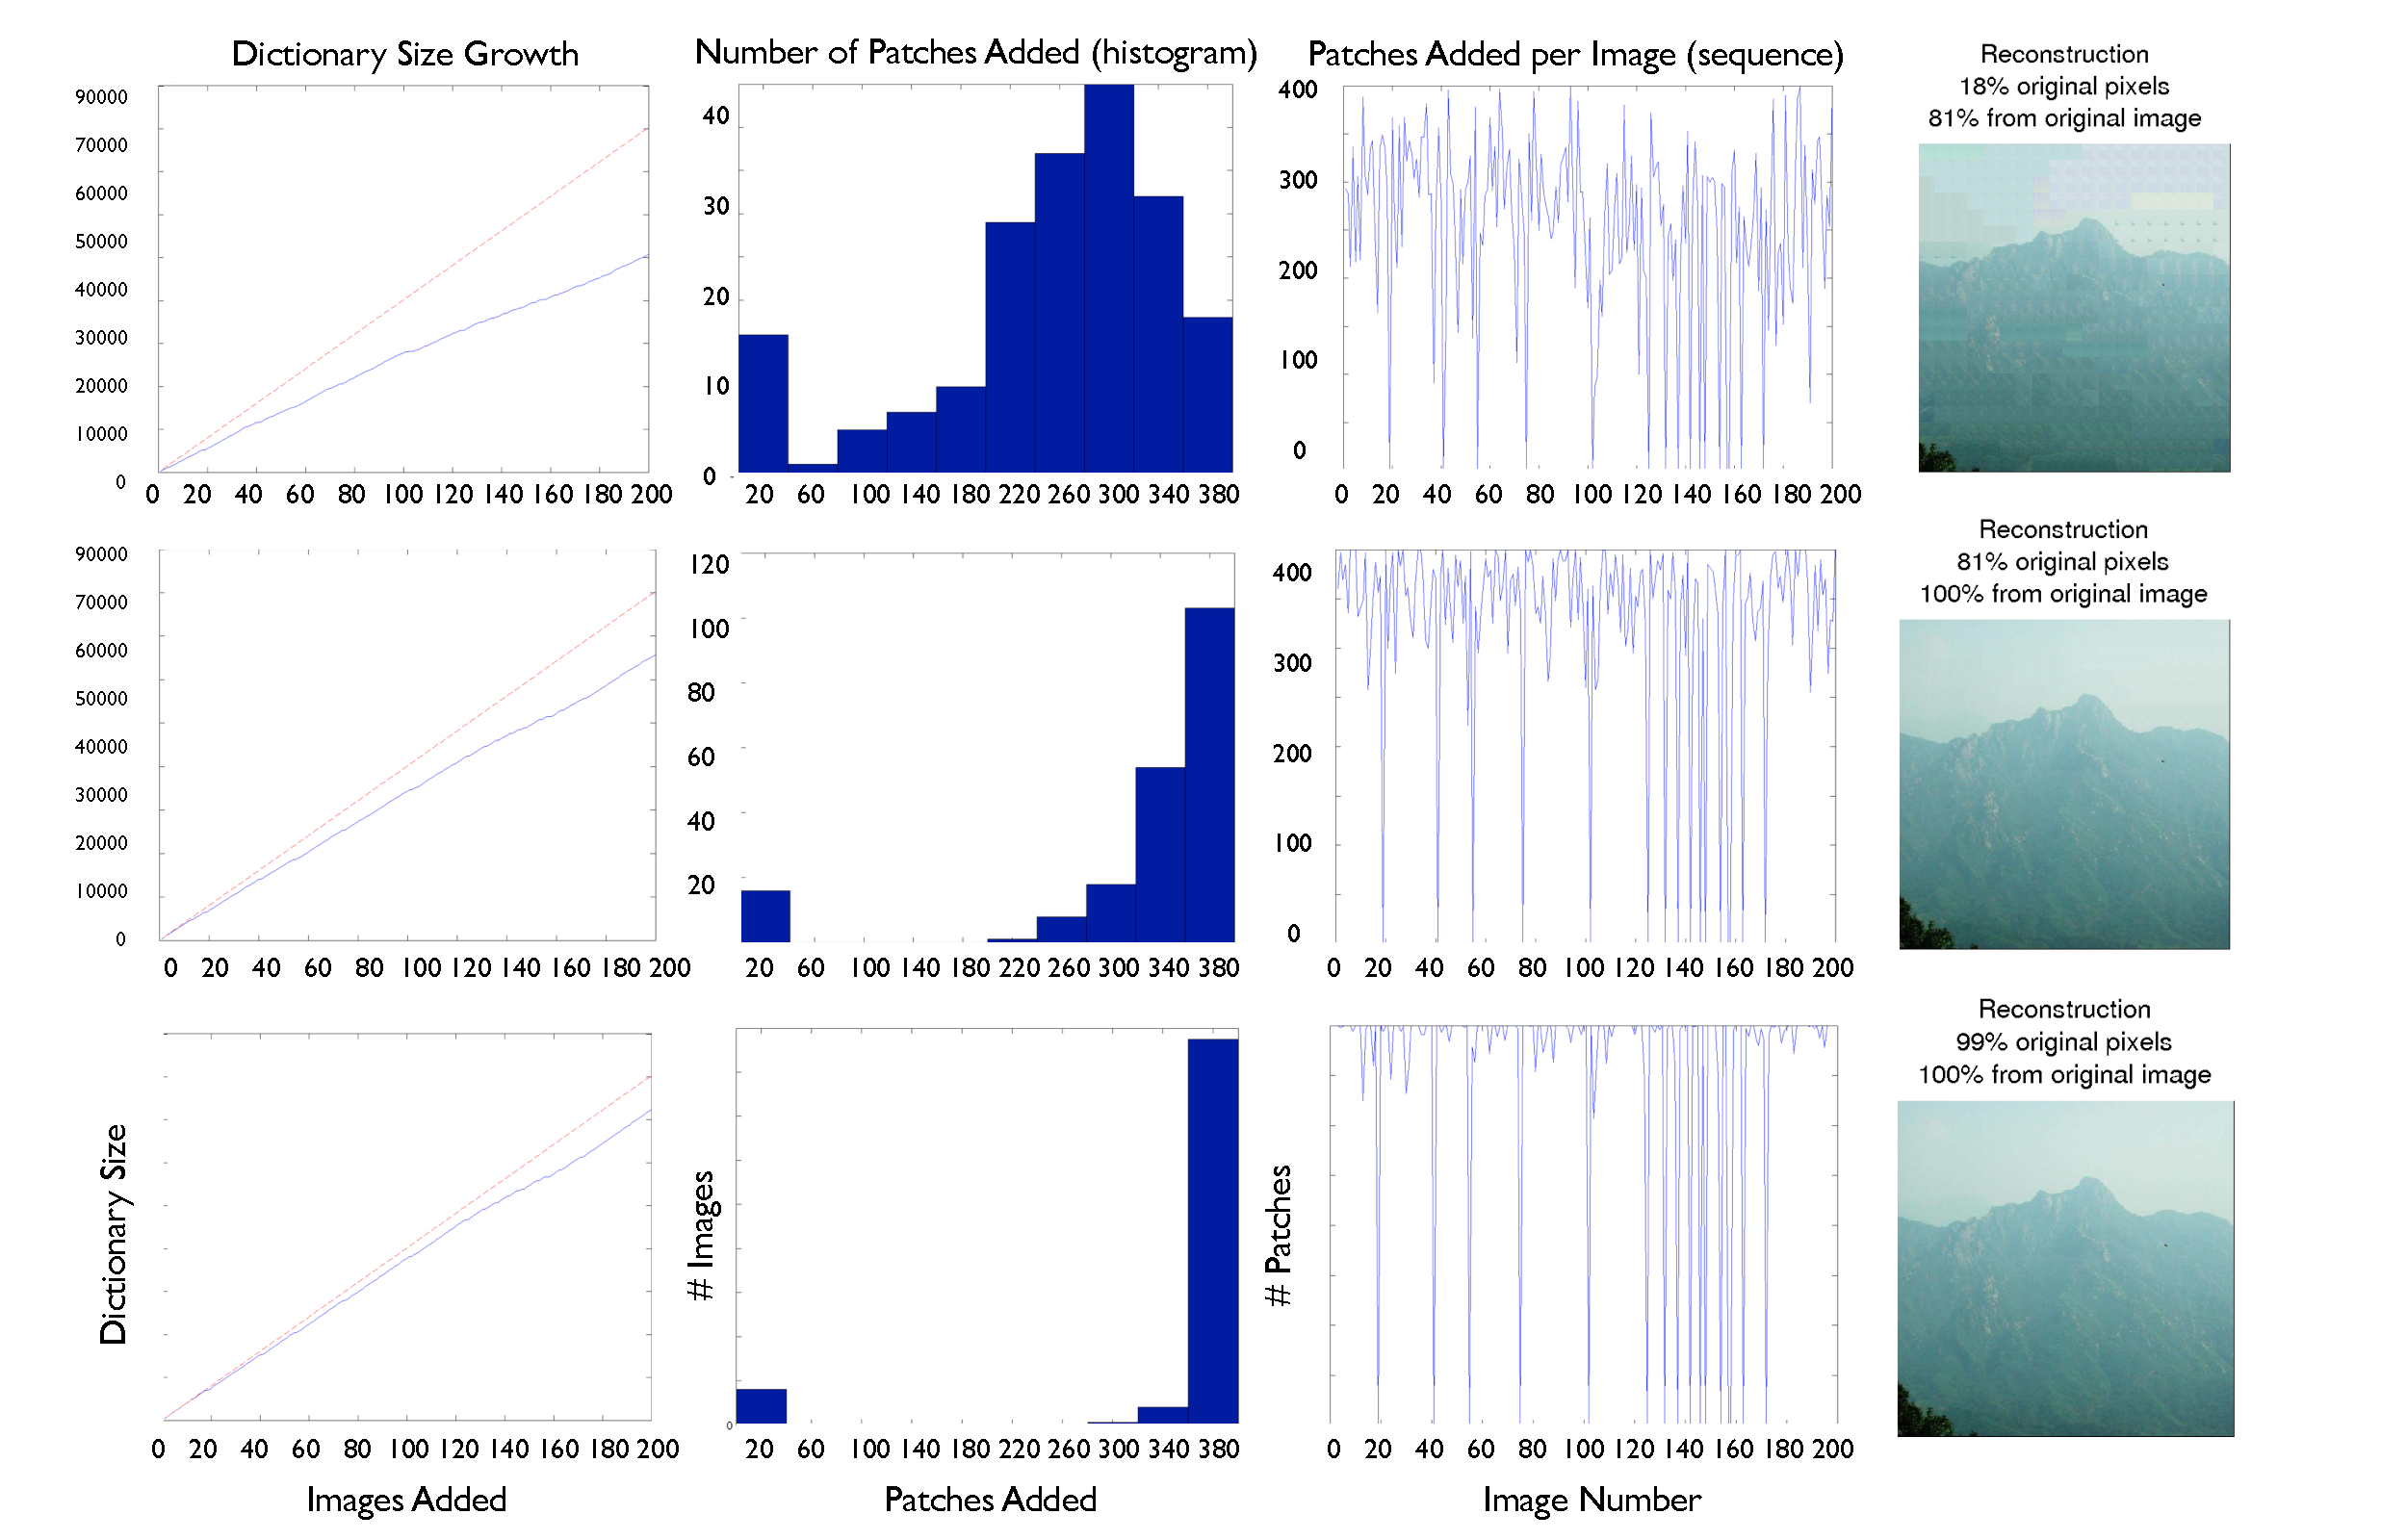
\includegraphics[width=1\linewidth]{Figures/perfGraphs_25_big.pdf}
\caption{Quantitative and qualitative results obtained by varying the patch distance threshold, $T$, while extracting $400$ patches from each image. In the first row, $T=0.1$, the dictionary size is 50,822 patches, and the average compression per image is $36.73\%$. In the second row, $T=0.01$, the dictionary size is $65,794$ patches, and the average compression per image is $18.09\%$. In the third row, $T=0.001$, the dictionary size is $72,445$ patches, and the average compression per image is $9.80\%$.}
\label{fig:perfGraphs}
\end{figure*}

